\documentclass[12pt]{report}
\usepackage{geometry}
\usepackage{graphicx}
\graphicspath{{images/}}
\textheight 600pt
\textwidth 440pt
\bibliographystyle{ieeetran}
\setlength{\parskip}{1em}

\begin{document}

\begin{titlepage}
    \begin{center}
        \vspace*{1cm}
        \Large
        \textbf{Automatic Detection and Classification of Diabetic Retinopathy Stages in Retinal Image}
        \normalsize
        \vspace{0.5cm}
        
        \vspace{1.5cm}
        
        \textbf{Author Name:}\\
        \textbf{Md. Abrar Labib (144423)}\\
        \textbf{Saquib Irtiza (144431)}\\
        
        \vfill
        
        \textbf{Supervisor Name:}\\
        \textbf{A.B.M. Ashikur Rahman}\\
        
        \vspace{0.6cm}
        
        
\includegraphics[width=0.3\textwidth]{iut}
        
        Islamic University of Technology (IUT)\\
        Computer Science and Engineering\\
        Bangladesh\\
        July, 2018
        
    \end{center}
\end{titlepage}
\Large
\begin{abstract}
\normalsize
\noindent This paper summarizes the different imaging techniques and methodologies used to perform classification of the different stages of a disease called diabetic retinopathy. In particular, it focuses on deep learning techniques to perform such detection in the fundus images of the patient's eye. Diabetic retinopathy is a progressive disease that causes the patient to lose eyesight if not diagnosed and treated at an early stage. Ophthalmologists usually diagnose the patient of this disease by screening the retinal fundus images to look for lesions. But the inaccuracy of such diagnosis together with the delay between diagnosis and treatment motivated researchers to automate this process of diagnosis. Using neural networks to train the system on a set of training images, it is possible to make systems that are more accurate and faster than human experts.  
\end{abstract}



\normalsize
\tableofcontents
\setlength{\parskip}{1em}

\chapter{Introduction}
\section{General Overview}
fff
\cite{kauppi2006diaretdb0}
\cite{kalviainen2007diaretdb1}
\cite{decenciere_feedback_2014}
\cite{kaggle_data}
\newpage
\section{Motivation}
\section{Purpose of this report}
\chapter{Diabetic Retinopathy}
\section{Stages of Diabetic Retinopathy}
fff
\newpage
\section{Image Dataset Available}


\chapter{Literature Review}
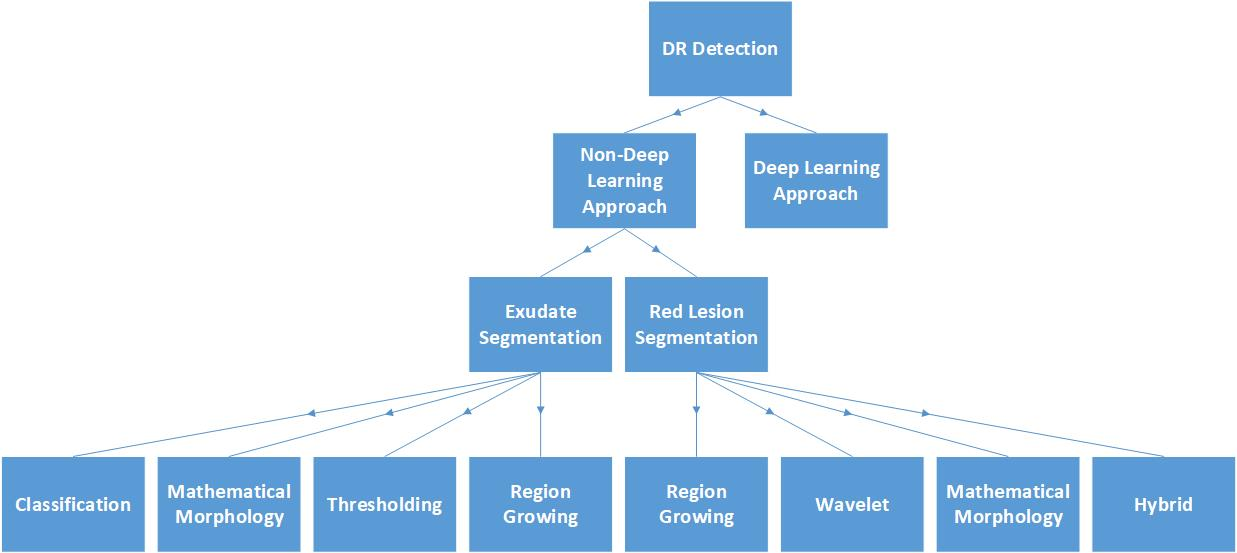
\includegraphics[width=1\textwidth]{Drawing1}

\section{Non Deep-Learning Methods}
Most non-deep learning approaches consist of several steps. Preprocessing steps such as contrast enhancement are usually carried out initially to lessen image variation by normalizing the original retinal image. Afterwards, irrelevant anatomical components such as the optic disk and vessels are removed. Finally, only the remaining pathological features of DR are retained for subsequent classification.

\noindent Non-deep learning methods from 2015 or earlier can be grouped into two types: exudate (EX) segmentation and red lesion (RL) segmentation.

\subsection{Exudate Segmentation}
EXs are lipoprotein intraretinal deposits due to vascular leakage. They appear in retinal images as yellowish lesions with well-defined edges. Their shape, size, brightness, and location vary among different patients. When clusters of EXs are located in the macular region, they are indicative of macular edema (ME), which is the main cause of visual loss in DR patients. For this reason, many researchers introduced the idea of a coordinate system based on the location of the fovea to determine DR grading. Different techniques have been proposed for EXs detection. They can be divided into four categories:

\subsubsection{■ Region Growing Method}
\subsubsection{o	Automated detection of diabetic retinopathy on digital fundus images (2008) \cite{sinthanayothin2002automated}.
}
\begin{itemize}
\item Authors: Sinthanayothin et al
\item Purpose: develop an automated screening system to analyse digital colour retinal images for important features of non-proliferative diabetic retinopathy (NPDR).
\item Method: High performance pre-processing of the colour images was performed. Previously described automated image analysis systems were used to detect major landmarks of the retinal image (optic disc, blood vessels and fovea). Recursive region growing segmentation algorithms combined with the use of a new technique, termed a ‘Moat Operator’, were used to automatically detect features of NPDR. These features included haemorrhages and microaneurysms (HMA), which were treated as one group, and hard exudates as another group.
\item Features:
\begin{itemize}
\item Hard exudates : identified as adjacent pixels with similar colour or grey level
\item HMA : sharpened using Moat Operator then identified by thresholding
\end{itemize}
\item Classifier: Multilayer perceptron neural network to identify blood vessels
\item Data: 112 digital fundus images of patients attending a DR screening service
\item Results: sensitivity and specificity for exudate detection were 88.5\% and 99.7\%
\end{itemize}

\subsubsection{■ Thresholding Method}
\subsubsection{o	Detection of exudates in retinal images using a pure splitting technique (2010) \cite{jaafar2010detection}.
}
\begin{itemize}
\item Authors: Jaafar et al
\item Method: an adaptive thresholding based on a novel algorithm for pure splitting of the image is proposed. A coarse segmentation based on the calculation of a local variation for all image pixels is used to outline the boundaries of all candidates which have clear borders. A morphological operation is used to refine the adaptive thresholding results based on the coarse segmentation results
\item Features:
\begin{itemize}
\item Exudates : local variation for each pixel of exudate region with clear margins
\item o	Non-exudates : discriminated using major axis length, minor axis length, area, solidity
\end{itemize}
\item Data: 50 abnormal images from DIARETDB0 database screening service
\item Results: 91.2\% sensitivity, 99.3\% specificity
\end{itemize}

\subsubsection{o	A novel automatic image processing algorithm for detection of hard exudates based on retinal image analysis (2008) \cite{sanchez2008novel}.
}
\begin{itemize}
\item Authors: Sanchez et al
\item Method: based on Fisher’s linear discriminant analysis and makes use of colour information to perform the classification of retinal exudates.
\item Features:
\begin{itemize}
\item Hard exudates : modified RGB model
\item Non-exudates : selecting pixels around optic disk depending on its area
\end{itemize}
\item Classifier: Fisher’s linear discriminant (FLD)
\item Data: 58 retinal images with variable colour, brightness, and quality
\item Results: sensitivity of 88\% using the lesion-based performance evaluation criterion, and accuracy of 100\% (sensitivity of 100\% and specificity of 100\%) image-based classification
\end{itemize}

\subsubsection{■ Mathematical Morpholopy Methods}
\subsubsection{o	Exudate detection in color retinal images for mass screening of diabetic retinopathy (2014). \cite{zhang2014exudate}}
\begin{itemize}
\item Authors: Zhang et al
\item Purpose: automatically detect normal exams in a tele-ophthalmology network, thus reducing the burden on the readers
\item Method: new preprocessing methods, which perform not only normalization and denoising tasks, but also detect reflections and artifacts in the image. A new candidates segmentation method, based on mathematical morphology. These candidates are characterized using classical features, but also novel contextual features. A random forest algorithm is used to detect the exudates among the candidates
\item Features:
\begin{itemize}
\item Contextual : distance between barycenter of candidate to nearest vessel, minimum distance of candidate to nearest vessel
\item Ultimate opening, a multi-scale morphological operator
\item Mean value of normalized saturation channel of each exudate candidate
\end{itemize}
\item Classifier: Random forest method
\item Data: A new clinical database, e-ophtha EX, containing precisely manually contoured exudates. It is very heterogeneous. It contains images gathered within the OPHDIAT telemedicine network for diabetic retinopathy screening
\item Results: AUC between 0.93 and 0.95
\end{itemize}

\subsubsection{o	Automatic detection of diabetic retinopathy exudates from non-dilated retinal images using mathematical morphology methods (2008). \cite{sopharak2008automatic}}
\begin{itemize}
\item Authors: Sopharak et al
\item Method: Preprocessing (RGB to HIS, median filter, contrast enhancement, optic disc elimination), exudates detection (closing, local variation, thresholding, morphological reconstruction)
\item Features:
\begin{itemize}
\item Exudate detection : size of structuring element in dilation, window size in local variation operator, threshold valued calculated using Otsu algorithm
\item Macular detection : Applying closing operator then thresholding
\end{itemize}
\item Data: All digital retinal images were taken from patients with nondilated pupils taken at Thammasat University Hospital
\item Results: Results: sensitivity and specificity are 80\% and 99.5\%
\end{itemize}

\subsubsection{■ Classification Method}
\subsubsection{o	A computational-intelligence-based approach for detection of exudates in diabetic retinopathy images (2009). \cite{osareh2009computational}}
\begin{itemize}
\item Authors: Osareh et al
\item Objective: Automated identification of exudate pathologies in retinopathy images based on computational intelligence techniques.
\item Method: The color retinal images are segmented using fuzzy c-means clustering following some preprocessing steps, i.e., color normalization and contrast enhancement. The entire segmented images establish a dataset of regions. To classify these segmented regions into exudates and nonexudates, a set of initial features such as color, size, edge strength, and texture are extracted. A geneticbased algorithm is used to rank the features and identify the subset that gives the best classification results. The selected feature vectors are then classified using a multilayer neural network classifier.
\item Features:
\begin{itemize}
\item Exudate discrimination : compactness of region, region size, region edge strength, mean Luv values inside and outside the region and Gabor filter response features
\end{itemize}
\item Classifier: three-layer perceptron NN with 65 node input
\item Data: large image dataset consisting of 300 manually labeled retinal images
\item Results: 96.0\% sensitivity, 94.6\% specificity
\end{itemize}

\subsubsection{o	Neural network based detection of hard exudates in retinal images (2009). \cite{garcia2009neural}}
\begin{itemize}
\item Authors: Garcia et al
\item Method: an algorithm which includes a neural network (NN) classifier. Three NN classifiers were investigated: multilayer perceptron (MLP), radial basis function (RBF) and support vector machine (SVM)
\item Features:
\begin{itemize}
\item Exudates : mean RGB values inside and outside the region and their standard deviations, region size, compactness and edge strength
\end{itemize}
\item Data: 117 images with variable colour, brightness, and quality. 50 of them (from DR patients) were used to train the NN classifiers and 67 (40 from DR patients and 27 from healthy retinas) to test
\item Results: Using a lesion-based criterion, a mean sensitivity (SEl) of 88.14\% and a mean positive predictive value (PPVl) of 80.72\% for MLP. With RBF, SEl = 88.49\% and PPVl = 77.41\%, while SEl = 87.61\% and PPVl = 83.51\% using SVM
\end{itemize}

\subsubsection{o    Automated detection of exudates for diabetic retinopathy screening (2007). \cite{fleming2007automated}}
\begin{itemize}
\item Authors: Fleming et al
\item Method: Candidate exudates were detected using a multi-scale morphological process. Based on local properties, the likelihoods of a candidate being a member of classes exudate, drusen or background were determined. This leads to a likelihood of the image containing exudates which can be thresholded to create a binary decision
\item Features:
\begin{itemize}
\item Exudate candidate : normalized luminosity and its standard deviation, normalized boundary gradient, candidate area, distance from nearest MA detected, and standardized colour features
\end{itemize}
\item Classifier: SVM having radial basis function kernel
\item Data: 13 219 images of which 300 contained exudates
\item Results: sensitivity 95.0\% and specificity 84.6\%
\end{itemize}

\subsubsection{o    Automated Detection and Differentiation of Drusen, Exudates, and Cotton-Wool Spots in Digital Color Fundus Photographs for Diabetic Retinopathy Diagnosis (2007). \cite{niemeijer2007automated}}
\begin{itemize}
\item Authors: Niemeijer et al
\item Purpose: To describe and evaluate a machine learning–based, automated system to detect exudates and cotton-wool spots in digital color fundus photographs and differentiate them from drusen, for early diagnosis of diabetic retinopathy
\item Method: : Each pixel was classified, resulting in a so-called lesion probability map that indicates the probability that a pixel is part of a bright lesion. Pixels with high probability were grouped into probable lesion pixel clusters. Based on cluster characteristics each probable lesion pixel cluster was assigned a probability indicating the likelihood that the pixel cluster was a true bright lesion. Each bright lesion cluster likely to be a bright lesion was classified as exudate, cotton-wool spot or drusen.
\item Features:
\begin{itemize}
\item True bright lesion detection : area, perimeter, compactness, length, width, mean gradient, mean of green channel pixels, mean CIE-LUV intensities, local pixel contrast, distance to closest red lesion
\end{itemize}
\item Classifiers: k-NN and a linear discriminant analysis classifier
\item Data: Three hundred retinal images from one eye of 300 patients with diabetes were selected from a diabetic retinopathy telediagnosis database (nonmydriatic camera, two-field photography): 100 with previously diagnosed bright lesions and 200 without
\item Results: The system achieved an area under the receiver operating characteristic (ROC) curve of 0.95 and sensitivity/specificity pairs of 0.95/0.88 for the detection of bright lesions of any type
\end{itemize}

\subsection{Red Lesion Segmentation}
MAs are small saccular bulges in the walls of retinal capillary vessels. In color fundus images, MAs appear like round red dots with a diameter ranging from 10 to 100 µm. MAs are difficult to distinguish from dot-HEMs, which are a little bigger. MAs are normally the first retinal lesions that appear in DR and their number has a direct relationship to DR severity. Several approaches have been proposed for MAs segmentation through color image analysis. The techniques for RL detection can be also divided into four categories:

\subsubsection{■ Region Growing Methods}
\subsubsection{o    Automated microaneurysm detection using local contrast normalization and local vessel detection (2006). \cite{fleming2006automated}}
\begin{itemize}
\item Authors: Fleming et al
\item Method: Various methods for contrast normalization are compared. Best results were obtained with a method that uses the watershed transform to derive a region that contains no vessels or other lesions. Dots within vessels are handled successfully using a local vessel detection technique
\item Features: number of peaks in smoothed energy function, major axis length, eccentricity of the elliptical cross section of the paraboloid, depth of the candidate, energy at the boundary
\item Classifier: k-NN with k = 15
\item Data: images acquired from diabetic patients attending the Grampian Diabetes Retinal Screening Programme 1441 images were graded by a clinician for the presence of MAs
\item Results: sensitivity 85.4\% and specificity 83.1\%
\end{itemize}

\subsubsection{■ Mathematical Morphology Methods}
\subsubsection{o   Automated microaneurysm detection method based on eigenvalue analysis using hessian matrix in retinal fundus images (2013). \cite{inoue2013automated}}
\begin{itemize}
\item Authors: Inoue et al
\item Method: After image preprocessing, the MA candidate regions were detected by eigenvalue analysis using the Hessian matrix in green-channeled retinal fundus images. Then, 126 features were calculated for each candidate region. By a threshold operation based on feature analysis, false positive candidates were removed. The candidate regions were then classified either as MA or false positive using artificial neural networks (ANN) based on principal component analysis (PCA). The 126 features were reduced to 25 components by PCA, and were then inputted to ANN
\item Features: based on pixel value, shape, texture analysis, reduced using principal component analysis (PCA)
\item Classifier: Classifier: artificial neural network (ANN)
\item Data: 25 retinal images from the retinopathy online challenge (ROC) database
\item Results: true positive rate was 73%, with eight false positives per image
\end{itemize}

\subsubsection{o  Automated detection of red lesions from digital colour fundus photographs (2011). \cite{jaafar2011automated}}
\begin{itemize}
\item Authors: Jaafar et al
\item Method: After pre-processing, a morphological technique was used to segment red lesion candidates from the background and other retinal structures. Then a rule-based classifier was used to discriminate actual red lesions from artifacts. A novel method for blood vessel detection is also proposed to refine the detection of red lesions
\item Features: aspect ratio, area, perimeter, circularity, eccentricity, mean intensity, inner standard deviation
\item Classifier: Rule-based classifier
\item Data: standarised test set of 219 images
\item Results: sensitivity of 89.7\% and a specificity of 98.6\% (at lesion level)
\end{itemize}

\subsubsection{o  Detection of microaneurysms using multi-scale correlation coefficients (2010). \cite{zhang2010detection}}
\begin{itemize}
\item Authors: Zhang et al
\item Method: a new approach based on multi-scale correlation filtering (MSCF) and dynamic thresholding is developed. This consists of two levels, microaneurysm candidate detection (coarse level) and true microaneurysm classification (fine level)
\item Features: area, perimeter, aspect ratio, circularity of the candidate, total, average and normalized intensities, compactness
\item Classifier: Discrimination table
\item Data: ROC (retinopathy on-line challenge) and DIARETDB1 (standard diabetic retinopathy database)
\item Results: 2nd rank in ROC competition
\end{itemize}


\subsubsection{o   Automatic detection of microaneurysms in color fundus images (2007). \cite{walter2007automatic}}
\begin{itemize}
\item Authors: Walter et al
\item Method: The first step consists in image enhancement, shade correction and image normalization of the green channel. The second step aims at detecting candidates, i.e. all patterns possibly corresponding to MA, which is achieved by diameter closing and an automatic threshold scheme. Then, features are extracted, which are used in the last step to automatically classify candidates into real MA and other objects; the classification relies on kernel density estimation with variable bandwidth
\item Features: no. of pixels in region, circularity, mean and maximal values of top-hat, dynamic (a classical morphological contrast measure), outer and inner grey level mean and standard deviation, grey level contrast, colour contrast
\item Classifier: KNN
\item Data: 21 annotated images Grampian Diabetes Retinal Screening Programme 1441 images were graded by a clinician for the presence of MAs
\item Results: sensitivity was 88.5\% at an average number of 2.13 false positives per image
\end{itemize}

\subsubsection{■ Wavelet-Based Method}
\subsubsection{o    Optimal wavelet transform for the detection of microaneurysms in retina photographs (2008). \cite{quellec2008optimal}}
\begin{itemize}
\item Authors: Quellec et al
\item Method: MAs are detected by locally matching a lesion template in subbands of wavelet transformed images. To improve the method performance, the best adapted wavelet within the lifting scheme framework is used. The optimization process is based on a genetic algorithm followed by Powell’s direction set descent
\item Data: 120 retinal images analyzed by an expert
\item Results: sensitivity of 89.62\%, positive predictive value of 89.50\%
\end{itemize}

\subsubsection{■ Hybrid Methods}
\subsubsection{o   Retinal Microaneurysm Detection Through Local Rotating Cross-Section Profile Analysis (2013). \cite{lazar2013retinal}}
\begin{itemize}
\item Authors: Lazar et al
\item Method: MA detection through the analysis of directional cross-section profiles centered on the local maximum pixels of the preprocessed image. Peak detection is applied on each profile, and a set of attributes regarding the size, height, and shape of the peak are calculated subsequently. The statistical measures of these attribute values as the orientation of the cross-section changes constitute the feature set that is used in a naïve Bayes classification to exclude spurious candidates. A formula for the final score of the remaining candidates is given, which can be thresholded further for a binary output
\item Features: increasing and decreasing ramp height, ramp slope, top and peak width, peak height
\item Classifier: Naïve Bayes classifier
\item Data: The ROC publicly available dataset consisting of 50 training and 50 test images
\item Results: overall score of 0.423, ranked 2nd in ROC competition
\end{itemize}

\subsubsection{o   Assessment of four neural network based classifiers to automatically detect red lesions in retinal images (2010). \cite{garcia2010assessment}}
\begin{itemize}
\item Authors: Garcia et al
\item Objective: detect red lesions (RLs), like haemorrhages and microaneurysms
\item Method: extracted a set of colour and shape features from image regions and performed feature selection using logistic regression. Four neural network (NN) based classifiers were subsequently used to obtain the final segmentation of RLs: multilayer perceptron (MLP), radial basis function (RBF), support vector machine (SVM) and a combination of these three NNs using a majority voting (MV) schema
\item Features: Region size, mean and standard deviation of RGB values in and around the region, compactness, edge strength, homogeneity, colour difference, circularity, eccentricity, aspect ratio
\item Classifiers: MLP, RBF, SVM
\item Data: 115 images divided into a training set of 50 images (with RLs) and a test set of 65 images (40 with RLs and 25 without RLs)
\item Results: best results were obtained for RBF. Using a lesion-based criterion, a mean sensitivity of 86.01\% and a mean positive predictive value of 51.99\% were obtained. With an image-based criterion, a mean sensitivity of 100\%, mean specificity of 56.00\%
\end{itemize}

\subsubsection{o   Mixture model-based clustering and logistic regression for automatic detection of microaneurysms in retinal images (2009). \cite{sanchez2009mixture}}
\begin{itemize}
\item Authors: Sanchez et al
\item Method: a statistical approach based on mixture model-based clustering and logistic regression. The innovative segmentation approach based on a statistical mixture model based clustering allows a robust separation of the foreground and background scenes and, specifically, a segmentation of MAS in a totally unsupervised manner
\item Features: based on shape, colour, brightness, contrast
\item Classifier: logistic regression classifier
\item Data: public database proposed by the Retinal Online Challenge
\item Results: overall score in the ROC competition of 0.332404
\end{itemize}

\subsubsection{o   Automated microaneurysm detection method based on double-ring filter and feature analysis in retinal fundus images (2009). \cite{mizutani2009automated}}
\begin{itemize}
\item Authors: Mizutani et al
\item Method: After image preprocessing, candidate regions for microaneurysms were detected using a double-ring filter. Any potential false positives located in the regions corresponding to blood vessels were removed by automatic extraction of blood vessels from the images. Twelve image features were determined, and the candidate lesions were classified into microaneurysms or false positives using the rule-based method and an artificial neural network
\item Features: area, circularity, length to width ratio, mean value of red, green and blue bits, contrast
\item Classifier: rule-based method and a three-layered feed forward ANN with back propagation algorithm
\item Data: Retinopathy Online Challenge (ROC) database (50 training cases, 50 test cases)
\item Results: sensitivity for detecting microaneurysms was 65\% at 27 false positives per image
\end{itemize}

\subsubsection{o   Automatic detection of red lesions in digital color fundus photographs (2005). \cite{niemeijer2005automatic}}
\begin{itemize}
\item Authors: Niemeijer et al
\item Method: a new red lesion candidate detection system based on pixel classification. Using this technique, vasculature and red lesions are separated from the background of the image. After removal of the connected vasculature the remaining objects are considered possible red lesions. An extensive number of new features are added to those proposed by Spencer–Frame. The detected candidate objects are classified using all features and a k-nearest neighbor classifier
\item Features: area, perimeter, aspect ratio, circularity, total, mean and normalized intensities in green plane and shade corrected image, compactness, mean and standard deviation of filter outputs
\item Classifier: kNN, linear discriminant, quadratic discriminant
\item Data: 100 images and was used to train and test composed of data taken from a screening program.
\item Results: sensitivity of 100\% at a specificity of 87\%
\end{itemize}

\section{Deep Learning Methods}
“Feature engineering,” involves computing explicit features specified by experts, resulting in algorithms designed to detect specific lesions or predicting the presence of any level of diabetic retinopathy.5 Deep learning6 is a machine learning technique that avoids such engineering by learning the most predictive features directly from the images given a large data set of labeled examples. This technique uses an optimization algorithm called back-propagation to indicate how a machine should change its internal parameters to best predict the desired output of an image. Some of the papers using deep learning algorithms to create models are given in the following section.

\subsection{Convolutional Neural Network}


A convolutional neural network (CNN) is a class of deep, feed-forward artificial neural networks. CNNs use a variation of multilayer perceptrons via backpropagation designed to require minimal preprocessing. CNNs use relatively little pre-processing compared to other image classification algorithms. This means that the network learns the filters that in traditional algorithms were hand-engineered. This independence from prior knowledge and human effort in feature design is a major advantage.




\subsubsection{■ Segmentation Using CNN}
\subsubsection{o   Development and Validation of a Deep Learning Algorithm for Detection of Diabetic Retinopathy in Retinal Fundus Photographs (2016). \cite{gulshan2016development}}
\begin{itemize}
\item Authors: Varun Gulshan et al
\item Objective: To apply deep learning to create an algorithm for automated detection of diabetic retinopathy and diabetic macular edema in retinal fundus photographs.
\item Method: CNN was implemented using Inception-v3 architecture proposed by Szegedy et al. The optimization algorithm used to train the network weights was a distributed stochastic gradient descent implementation by Dean et al.16 To speed up the training, batch normalization7 as well as preinitialization using weights from the same network trained to classify objects in the ImageNet data set17 were used. An ensemble19 of 10 networks trained on the same data was used, and the final prediction was computed by a linear average over the predictions of the ensemble.
\item Data: The EyePACS-1 data set consisted of 9963 images and Messidor-2 data set had 1748 images
\item Result: The performance of the algorithm at the high-sensitivity and high-specificity operating points are:
\begin{itemize}
\item High-sensitivity operating point: specificity was 84.0\% and sensitivity was 96.7\%.
\item High-specificity operating point: specificity was 93.8\% and sensitivity was 90.7\%
\item The area under the receiver operating characteristic curve was 97.4\%
\end{itemize}
\end{itemize}

\subsubsection{o   Improved Automated Detection of Diabetic Retinopathy on a Publicly Available Dataset Through Integration of Deep Learning (2016). \cite{abramoff2016improved}}
\begin{itemize}
\item Authors: Michael David Abramoff  et al
\item Objective: To compare performance of a deep-learning enhanced algorithm for automated detection of diabetic retinopathy.
\item Method: A hybrid device applies a set of CNN-based detectors to each of the images in the exam. These detectors are trained and optimized to detect normal retinal anatomy, such as optic disc and fovea, as well as the lesions characteristic for DR, such as hemorrhages, exudates, and neovascularization. They are inspired by Alexnet23 and the Oxford Visual Geometry Group26 network architectures. The analysis software provides four types of outputs:
\begin{itemize}
\item Negative: implying no or only mild DR present
\item rDR: implying rDR is present
\item vtDR: implying vtDR is present
\item Low exam quality: implying either protocol errors or low quality of the individual images.
\end{itemize}
If the index is above or equal to the vtDR threshold, a positive output for vtDR is returned. If the vtDR index is below this threshold, the rDR index is thresholded. If the rDR index is above or equal to this latter threshold a positive output for rDR is returned. If it is below the latter threshold an output of ‘‘negative’’ is returned. The device was never trained on any of the Messidor-2 images.
\item Data: 10,000 to 1,250,000 unique samples, depending on the lesion to be detected are used for training. Messidor-2 data consisting of 1748 images is used for validation.
\item Result: The device with CNN based detectors performed pretty good with results of:
\begin{itemize}
\item vtDR: 100\% sensitivity, 91\% specificity and 0.989 AUC.
\item rDR: 96.8\% sensitivity and 87.0\% specificity
\item The area under the receiver operating characteristic curve was 97.4\%
\end{itemize}
\end{itemize}

\subsubsection{o Fast convolutional neural network training using selective data sampling: Application to hemorrhage detection in color fundus images (2016). \cite{van2016fast}}
\begin{itemize}
\item Authors: van Grinsven et al
\item Objective: a method to improve and speed-up the CNN training for medical image analysis tasks by dynamically selecting misclassified negative samples during training
\item Method: A dynamic CNN training strategy where informative normal samples are dynamically selected at each training epoch from a large pool of medical images. A dynamic weight is assigned to each pixel in the negative training pool indicating its informativeness level. After each CNN training epoch, the weight of each negative training pixel is updated. This process is repeated until a stopping criterion is reached. The final trained CNN is used to classify each pixel in the test images, resulting in a pixel probability map for each test image
\item Network details: The CNN architecture used in this study consists of five convolutional layers followed by rectified linear units (ReLUs) and spatial max-pooling. The final layers of the network consist of a fully connected layer and a final softmax classification layer.
\item Data: Kaggle and Messidor databases
\item Result: A decreased training time from 170 epochs to 60 epochs with an increased performance – on par with two human experts – was achieved with areas under the receiver operating characteristics curve of 0.894 and 0.972 on two data sets. The SeS CNN statistically outperformed the NSeS CNN on an independent test set
\end{itemize}

\subsubsection{o Convolutional Neural Networks for Diabetic Retinopathy (2016). \cite{pratt2016convolutional}}
\begin{itemize}
\item Authors: Pratt et al
\item Objective: A network with CNN architecture and data augmentation which can identify the intricate features involved in the classification task such as micro-aneurysms, exudate and haemorrhages on the retina and consequently provide a diagnosis automatically and without user input
\item Method: Preprocessing tasks such as colour normalization and resizing were performed. The network was trained using stochastic gradient descent with Nestrov momentum. Afterwards, real-time dataaugmentation was used throughout training to improve the localisation ability of the network
\item Network details:  The network starts with convolution blocks with activation and then batch normalisation after each convolution layer. As the number of feature maps increases they move to one batch normalisation per block. All maxpooling is performed with kernel size 3x3 and 2x2 strides. After the final convolutional block the network is flattened to one dimension. To avoid overfitting they used weighted class weights relative to the amount of images in each class. Likewise, they performed dropout on dense layers, to reduce overfitting, until they reached the dense five node classification layer which uses a softmax activation function to predict our classification. The leaky rectified linear unit13 activation function was used, applied with a value of 0.01, to stop over reliance on certain nodes in the network. Similarly, in the convolution layers, L2 regularisation was used for weight and biases. The network was also initialized with Gaussian initialisation to reduce initial training time. The loss function used to optimise was the widely used categorical cross-entropy function.
\item Data: Kaggle databases
\item Result: a sensitivity of 95\% and an accuracy of 75\% on 5,000 validation images
\end{itemize}

\subsubsection{o Improved Microaneurysm Detection using Deep Neural Networks (2016). \cite{haloi2015improved}}
\begin{itemize}
\item Authors: Haloi et al
\item Objective: a novel microaneurysm (MA) detection for early diabetic retinopathy screening using color fundus images
\item Method: Each pixel of the image is classified as either MA or non-MA using a deep neural network with dropout training procedure using maxout activation function. No preprocessing step or manual feature extraction is required
\item Network details: three convolutional layers each followed by a max-pooling layer and one fully connected layer. And a softmax layer on the top of the network with two neurons for MA and non-MA probability values
\item Data: Retinopathy Online Challenge (ROC) and Diaretdb1v2 database
\item Result: accuracy of 95\% with sensitivity and specificity of 97\% and 94\% respectively on Messidor dataset
\end{itemize}

\subsubsection{o Automated Identification of Diabetic Retinopathy Using Deep Learning (2017). \cite{gargeya2017automated}}
\begin{itemize}
\item Authors: Gargeya et al
\item Objective: to develop a data-driven deep learning algorithm to automate DR screening
\item Network details: convolutional parameter layers learn iteratively filters that transform input images into hierarchical feature maps, learning discriminative features at varying spatial levels without the need for manually tuned parameters. each convolutional layer used batch normalization and the ReLU nonlinearity function to ensure smooth training and prevent overfitting, while using 2-class categorical cross-entropy loss for class discrimination
\item Data: Messidor 2 and E-Optha databases
\item Result: a 0.94 and 0.95 AUC score
\end{itemize}

\chapter{Implementation and Future Work}
\section{Implementation}
Two implementations of diabetic retinopathy classification using CNN was attempted on a laptop computer having  
Core i7 2.6 GHz processor, 16 GB RAM and GTX 960M graphics card. These implementations were based on methods used by participants of Kaggle DR Classification Competition. The code was implemented using python programming language on ubuntu operating system. Library functions such as OpenCV, Theano, Lasagna and Tensorflow were used. Although the preprocessing scripts ran succesfully in our setup, the network scripts could not be implemented since out system wasnt powerful enough to handle such large amount of computation. We used Kaggle DR database for these implementation. 
\section{Future Works}
\begin{itemize}
\item Separation of training and validation datasets could be done before and after the augmentation to see how it performs.
\item Use different ensemble methods to merge the network formed by CNN to see which performs better.
\item Use the combination of layers in a neural network that gives a higher amount of accuracy for the dataset being used in the minimum amount of time and complexity.
\item Use different preprocessing steps that increase the accuracy of the model such as:
\begin{itemize}
\item Enhancement on images might enhance dirt on the lens making images of level 0 appear as level 4. So we need to compensate for this problem.
\item Images could be of different resolution. Enlarging all images to one common resolution might result in details to be lost. So we need to find optimum resolution for which the best accuracy is achieved.
\item There can be an unbalanced number of images in different classes. So we need to ensure consistency in the preprocessing step without overfitting.
\end{itemize}
\end{itemize}

\chapter{Conclusion}
As discussed in this report, many work related to this field have already been using deep learning and feature based learning. But still, there is a scope to further enhance the techniques to improve efficiency and the complexity of the algorithms. Further research is necessary to determine the feasibility of applying this algorithm in the clinical setting and to determine whether use of the algorithm could lead to improved care and outcomes compared with current ophthalmologic assessment. And it is also very important that we address this problem at hand fast since the predicted numbers of people being infected by this disease are increasing everyday.

\bibliography{Reference}




\end{document}